\chapter{Clean Architecture}
\section{Was ist Clean Architecture?}
% allgemeine Beschreibung der Clean Architecture in eigenen Worten
Die Clean Architecture ist ein Architekturmuster, das sich auf die Trennung von Verantwortlichkeiten und die Abhängigkeiten zwischen den Schichten konzentriert. Die Architektur besteht aus mehreren Schichten, die von innen nach außen, wie in Abbildung \ref{fig:cleanArchitecture} zu sehen, angeordnet sind:

\begin{figure}[h]
    \centering
    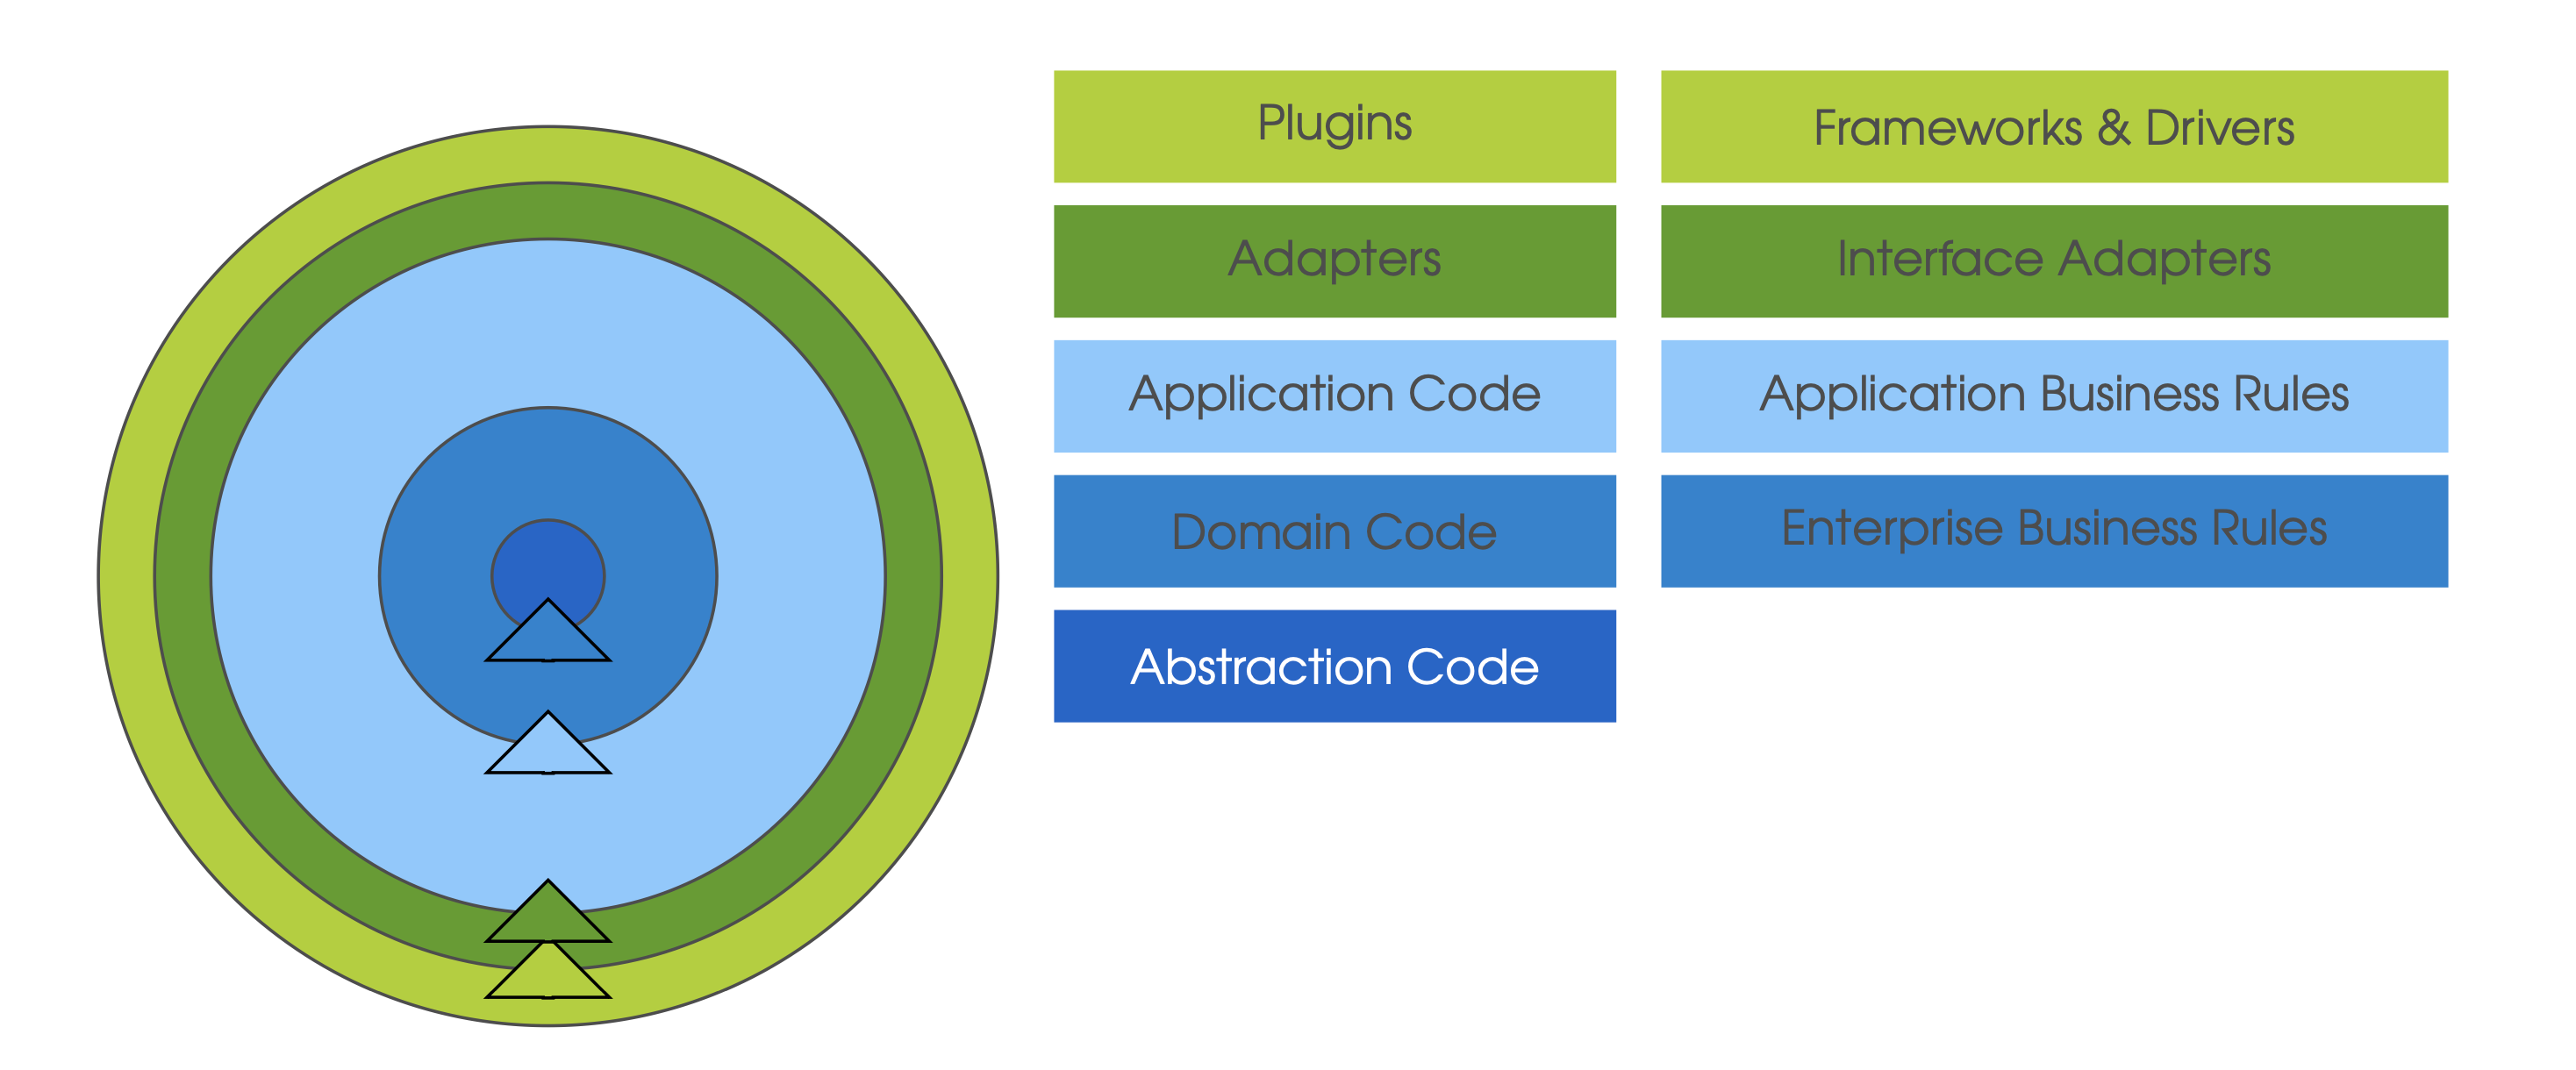
\includegraphics[width=0.8\textwidth]{Bilder/CA.png}
    \caption{Clean Architecture \cite{clean.2023}}
    \label{fig:cleanArchitecture}
\end{figure}

\begin{enumerate}
    \item \textbf{Abstraction Code (Schicht 4):} Code, welcher Konzepte, grundlegende Algorithmen und Datenstrukturen implementiert. Dieser Code enthält Domänen-übergreifendes Wissen und wird nur selten berührt.
    \item \textbf{Domain Code (Schicht 3):} Diese Schicht enthält die Kernlogik der Anwendung und wird am seltensten geändert. Hier werden die Geschäftsregeln und -modelle definiert. Die Entitäten der Domäne  werden von der Application Schicht verwendet.
    \item \textbf{Application Code (Schicht 2):} Diese Schicht enthält die Geschäftslogik der Anwendung(Use Cases welche direkt aus Anforderungen resultieren) und koordiniert den Datenfluss mit Hilfe der Entitäten der Domäne. Dabei sind die Regeln der anwendungsspezifischen Logik nicht projektweit gültig.  
    \item \textbf{Adapters (Schicht 1):}
    \item \textbf{Plugins(Schicht 0):}
\end{enumerate}
\section{Analyse der Dependency Rule}
% (1 Klasse, die die Dependency Rule einhält und eine Klasse, die die Dependency Rule verletzt);   jeweils UML der Klasse und Analyse der Abhängigkeiten in beide Richtungen (d.h., von wem hängt die Klasse ab und wer hängt von der Klasse ab) in Bezug auf die Dependency Rule

\subsection{Positiv-Beispiel: Dependency Rule}

\subsection{Negativ-Beispiel: Dependency Rule}

\section{Analyse der Schichten}
% jeweils 1 Klasse zu 2 unterschiedlichen Schichten der Clean-Architecture: jeweils UML der Klasse (ggf. auch zusammenspielenden Klassen), Beschreibung der Aufgabe, Einordnung mit Begründung in die Clean-Architecture
